

\chapter{Introduction to Functional MRI}\label{chap:intro_fmri}
\markright{{~{\rm \ref{chap:intro_fmri}}. Introduction to fMRI}\hfill}{}

\label{Chapter_1}



\vspace*{\fill}
\newthought{In this chapter} we introduce functional magnetic resonance imaging (fMRI). We will start by providing some insight into human brain structure and function. Then, we will introduce the principal brain imaging techniques in use nowadays. Different imaging techniques can be used to answer different neuroscientific questions. Functional MRI, due to its good spatial resolution and whole brain coverage is specially well suited to answer questions relating the localization of brain activity for a given task.

Before the data acquired through fMRI can be used in statistical analysis it has to go through a  preprocessing pipeline. In the last part of this chapter we detail the different steps of this pipeline, with special emphasis on the general linear model (GLM), a model that allows to extract time-independent activation coefficients from the fMRI time series in event-related designs.  These activation coefficients will form the basis of statistical studies presented in later chapters. 

% In the last part of the chapter we focus on fMRI and we relate the different steps from the scanner images to the statistical studies of later chapters.

% The objective of cognitive studies relating the brain's structure to its function is the output of time-independent activation maps for a given task. We will present a model, known as general linear model (GLM) .


% {\blue
% fMRI consist of successive  brain scans, given in intervals ranging from 1 to 4 seconds. However,  Because of the inherent delay of oxygen consumption in the brain, construction of these maps is not straightforward in the case of fMRI for fast event-related designs. We will describe a model known as general linear model (GLM) that .
% }

\hspace{20pt}
\minitoc
\vspace*{\fill}

\newpage


\section{General brain structures}\label{Chapter_1_Section_1}



The human brain has a volume of around $1200 \; cm^3$ and an average weight  of 1.5 kg. It is composed of neurons, glia cells and blood vessels. Glia cells are responsible for the structural and metabolic support of neurons. About $86$ billion neurons~\citep{Azevedo2009} process and transmit information through electrical and chemical signals. The information is transmitted along the neuron by \emph{action potentials}
(also called \emph{spikes}), that are short-lasting electrical events in which
the electrical membrane potential of a cell rapidly rises and falls. 

\begin{marginfigure}[-0.5cm]
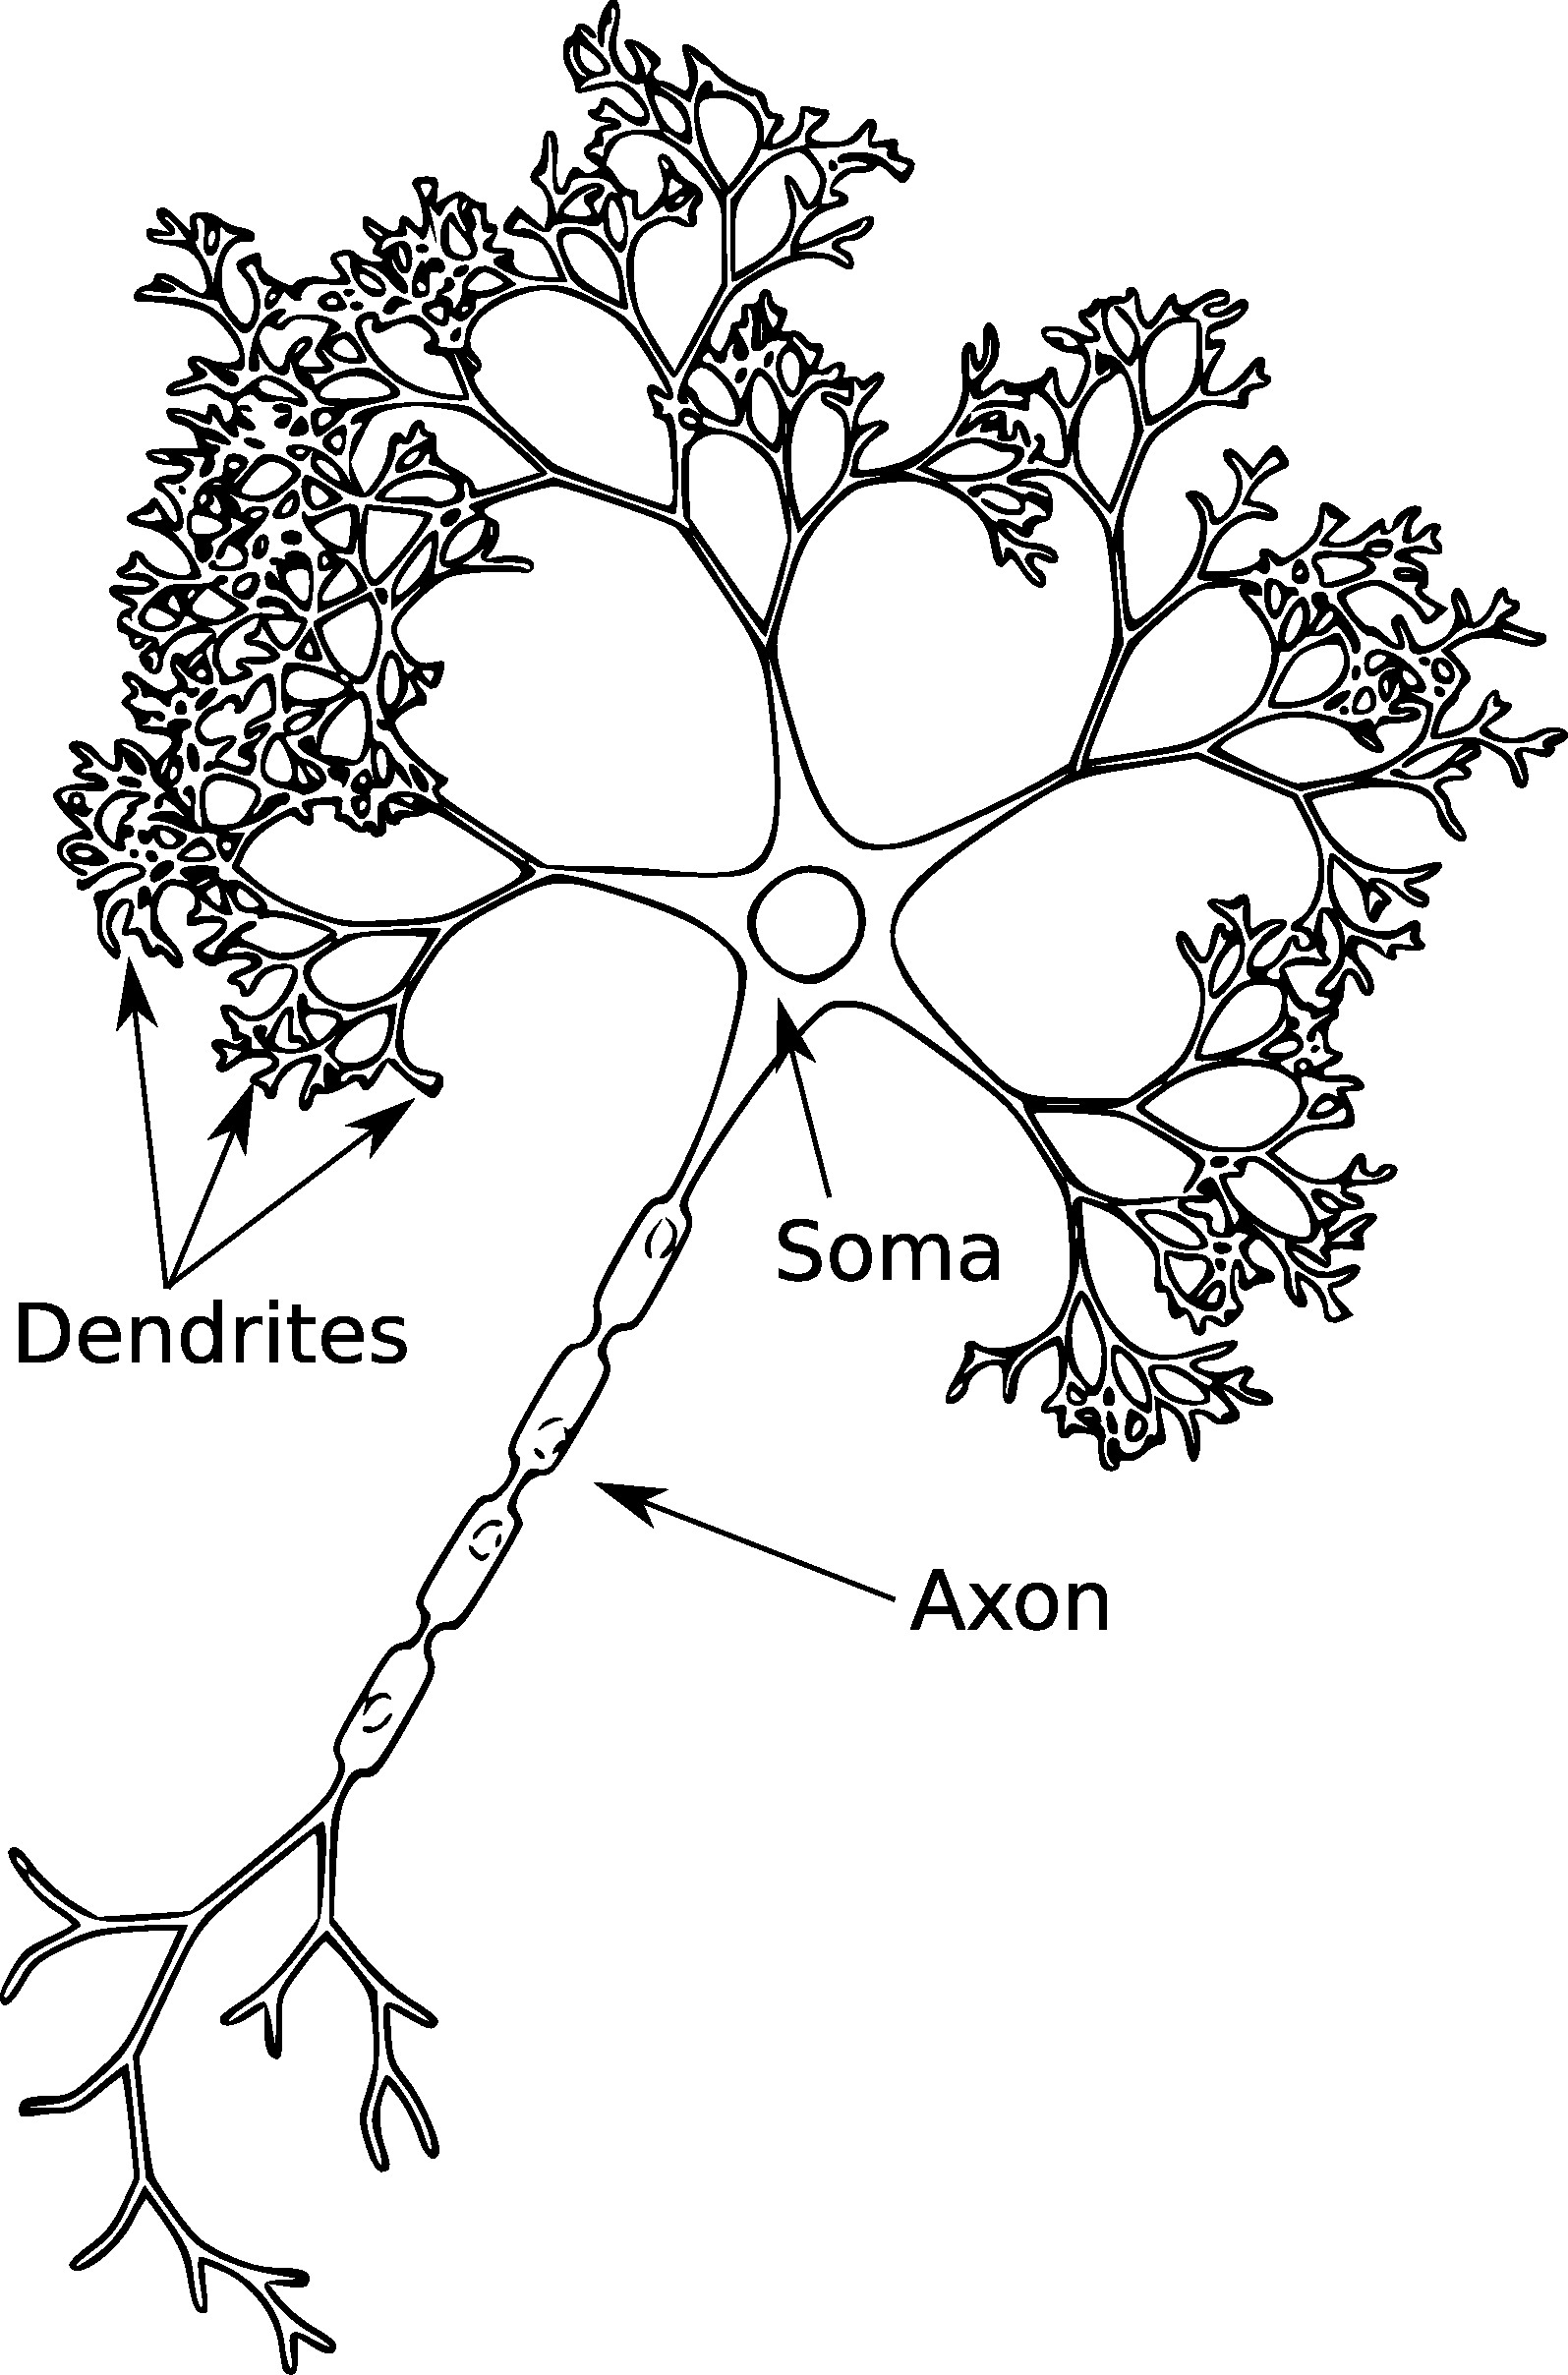
\includegraphics[width=1.0\linewidth]{chapter_1/chapter_1_neuron.pdf}
\vspace{-20pt}\caption{
Schematic view of a neuron, in scale $10^{5}:1$. A neuron has a cell body (\emph{soma}), many regions for receiving information from other neural cells (\emph{dentrites}) and often a nerve fiber called \emph{axon}.
Adapted from http://commons.wikimedia.org/.}\label{fig:chapter_1_neuron}
\end{marginfigure}


A neuron (Fig.~\ref{fig:chapter_1_neuron}) has a cell body (called the \emph{soma}), many regions for
receiving information from other neural cells (called \emph{dendrites}),
and
often an \emph{axon} (\emph{nerve fiber}) for transmitting information to
other
cells. Neurons communicate with one another via chemical synapses, where the axon terminal of one cell impinges upon another neuron's dendrite, soma or, less commonly, axon. Neurons can have over 1000 dentritic branches, making connections with tens of thousands of other cells. Synapses can be excitatory or inhibitory and either increase or decrease activity in the target neuron. Some neurons also communicate via electrical synapses, which are direct, electrically conductive junctions between cells.

\begin{marginfigure}[0.5cm]
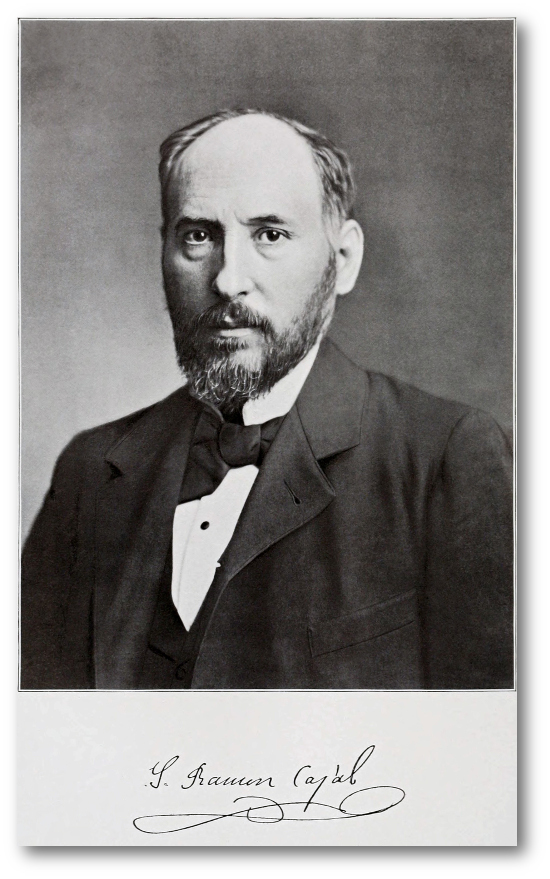
\includegraphics[width=1.\linewidth]{chapter_1/Cajal-shadow.jpg}
\vspace{-10pt}\caption{
	Santiago Ramón y Cajal (Navarre, Spain 1852 – Madrid, Spain 1934) is widely regarded as the father of modern neuroscience. Cajal and italian anatomist Camillo Golgi impersonated the dispute between neuron and reticular theory at the turn of the 20th century. They received a joint Nobel Prize in Physiology and Medicine in 1906.
}
\end{marginfigure}



The human brain can be decomposed in two parts: the \emph{white matter}, constituted by the nerve
fibers, and the \emph{gray matter} constituted by the neural cell bodies.
The surface of the human brain is a highly circonvoluted 6-layered structure
called \emph{neocortex} (or more simply \emph{cerebral cortex}). This layer is folded in a way that increases the amount of surface that can fit into the volume available. A cortical fold is called \emph{sulcus}, and the area between two \emph{sulci} is called a \emph{gyrus}.


The human cortex is often divided into four ``lobes'', called the frontal lobe, parietal lobe, temporal lobe and occipital lobe (see Figure~\ref{fig:chapter_1_functions}). The left and right side hemispheres of the cortex are broadly similar in shape, and most cortical areas are replicated on both sides. Some areas, however, show strong lateralization, such as areas that are involved in language, located in the vast majority of subject in the left hemisphere.

% \begin{marginfigure}
% 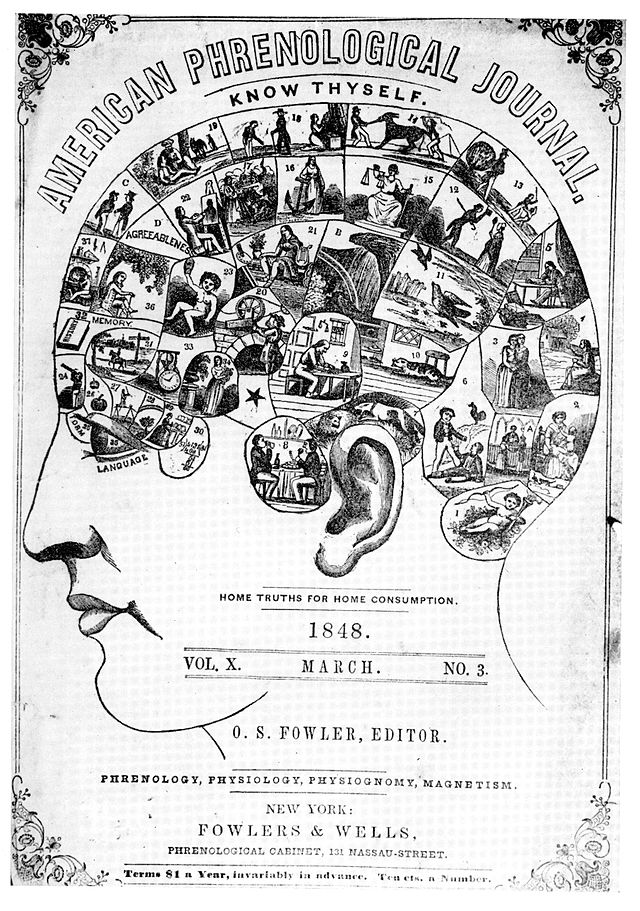
\includegraphics[width=1.\linewidth]{figures/640px-Phrenology-journal.jpg}
% \caption{Front page of the Americal Phrenological Journal, 1848. Although now considered a pseudoscience, phrenological thinking has been influential in 19th-century psychiatry and modern neuroscience}
% \end{marginfigure}

How the different anatomical structures of the brain correspond to the neural substrate of cognitive functions is one of the oldest debates in neuroscience, defining an entire field: cognitive neuroscience. The idea of linking a given cognitive function to a specific brain region can be traced back to the work of nineteen century phrenologists, who based their localizationist attempts on the shape of the skull. In the 20th century, a group of neuropsychologists, in absence of direct means to investigate brain activity, studied patients with cortical damages observing that some focal lesions were associated with relatively global effects on behavior. This lead them to argue against a strictly localizationist view of brain organization. Nowadays it is widely recognized that the activity of specific brain regions underlie many cognitive functions (e.g.vision, in occipital areas). At the same time, the relevance of \emph{brain networks} encompassing different anatomical regions for the multimodal integration of features necessary for higher level cognitive functions (e.g.attention in the fronto-parietal network) ~\citep{gazzaniga2004cognitive} has been acknowledged.


\begin{figure}
\begin{center}
\center 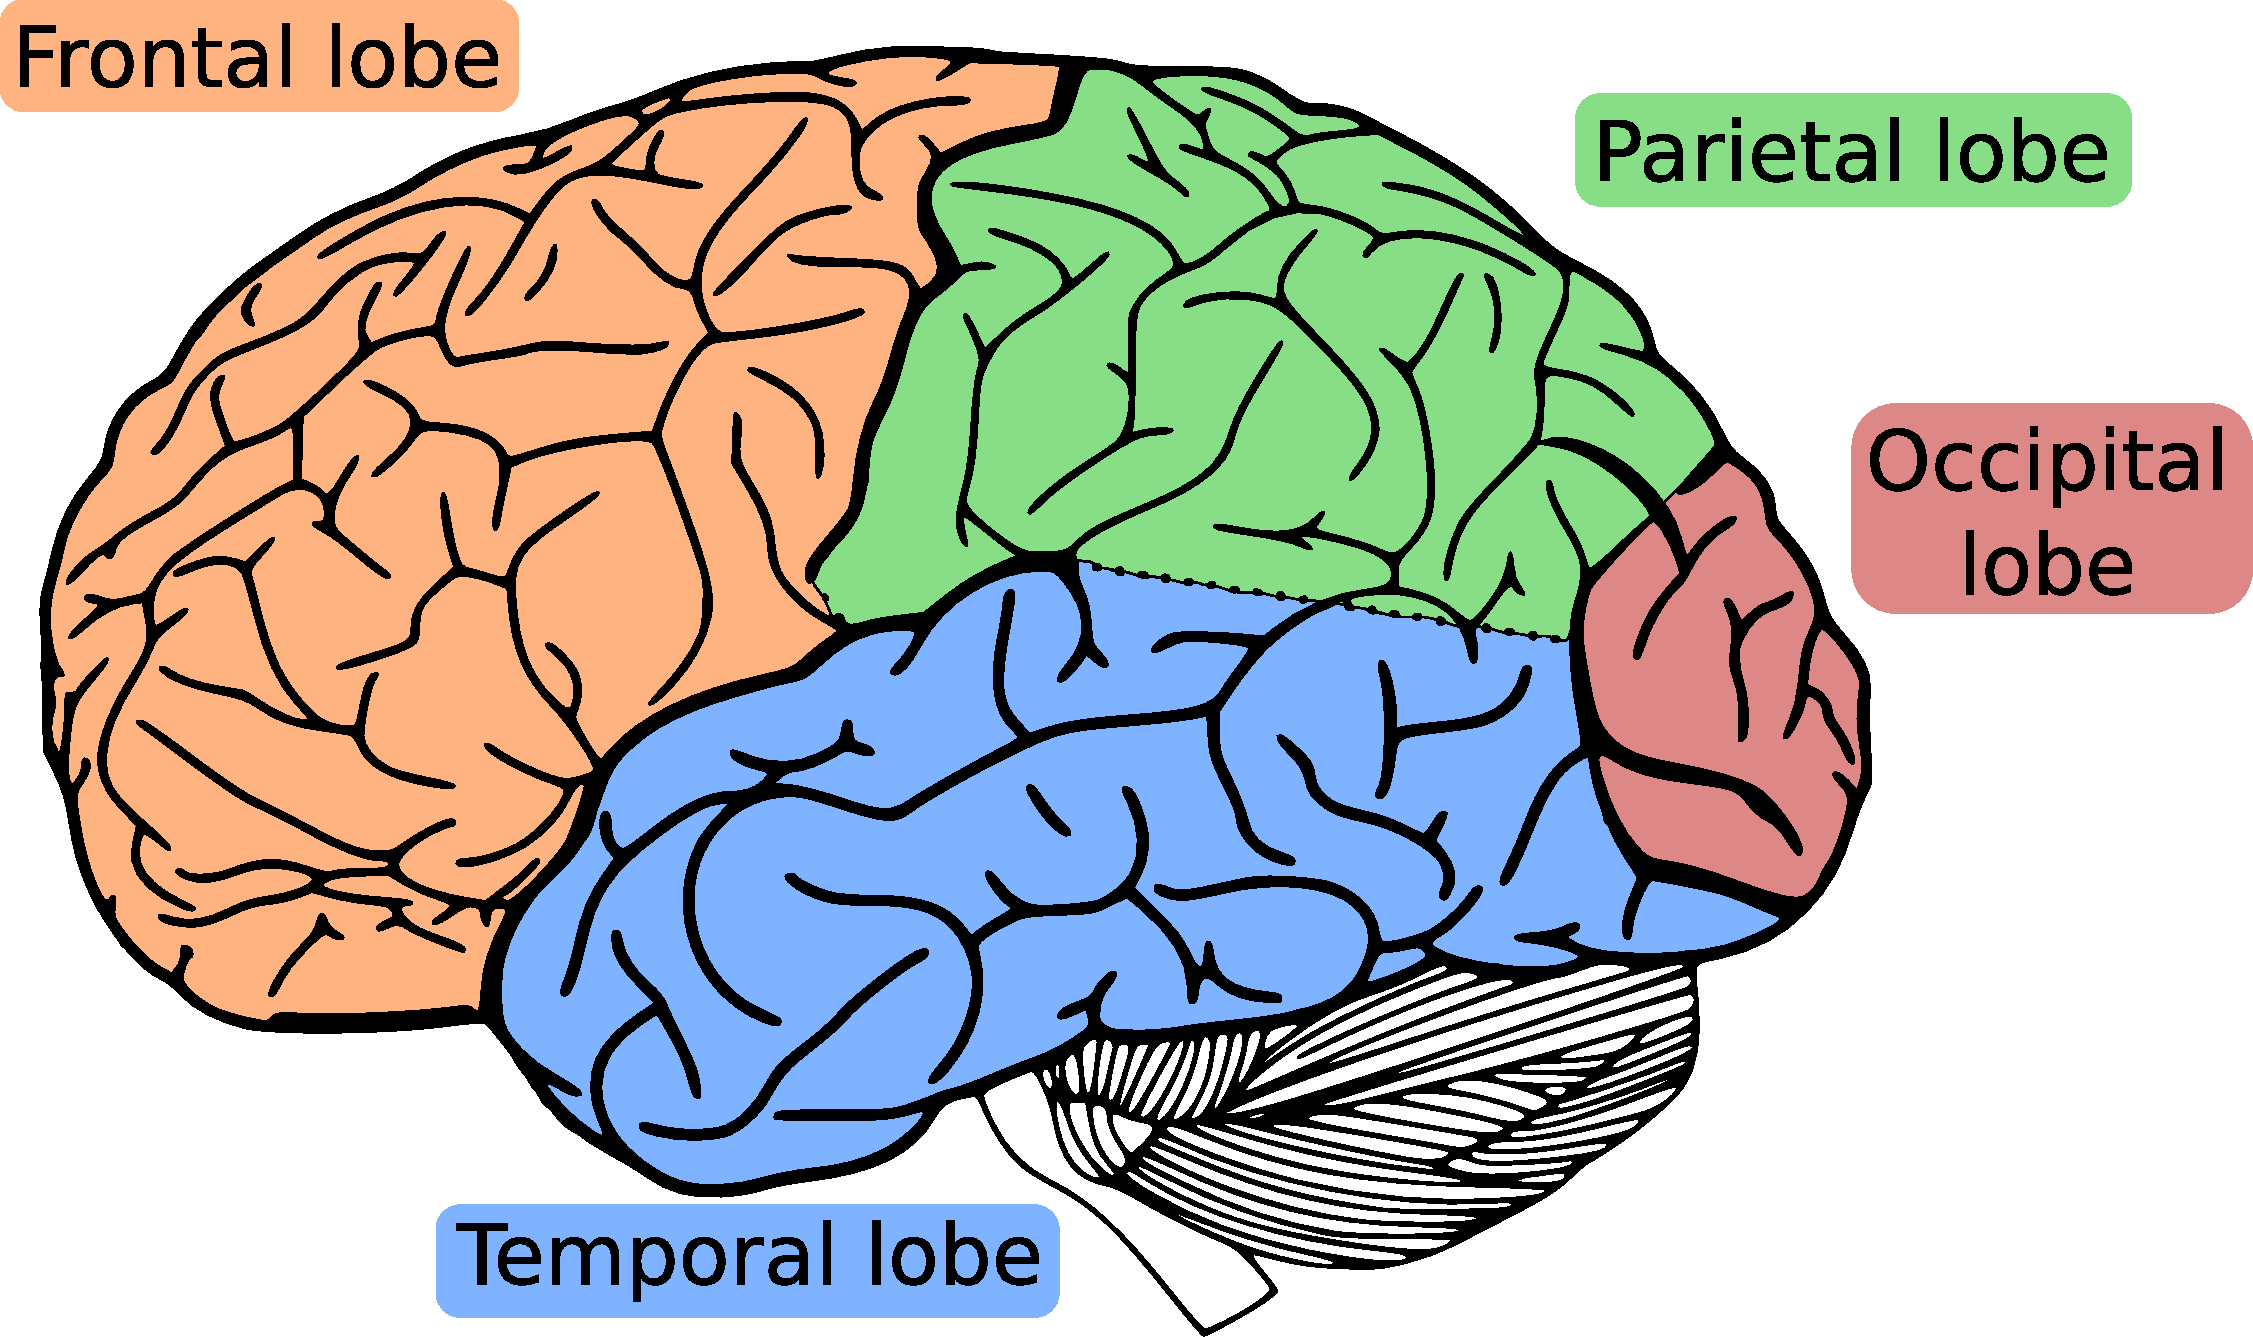
\includegraphics[width=0.6\linewidth]{chapter_1/chapter_1_lobe.pdf}
\center 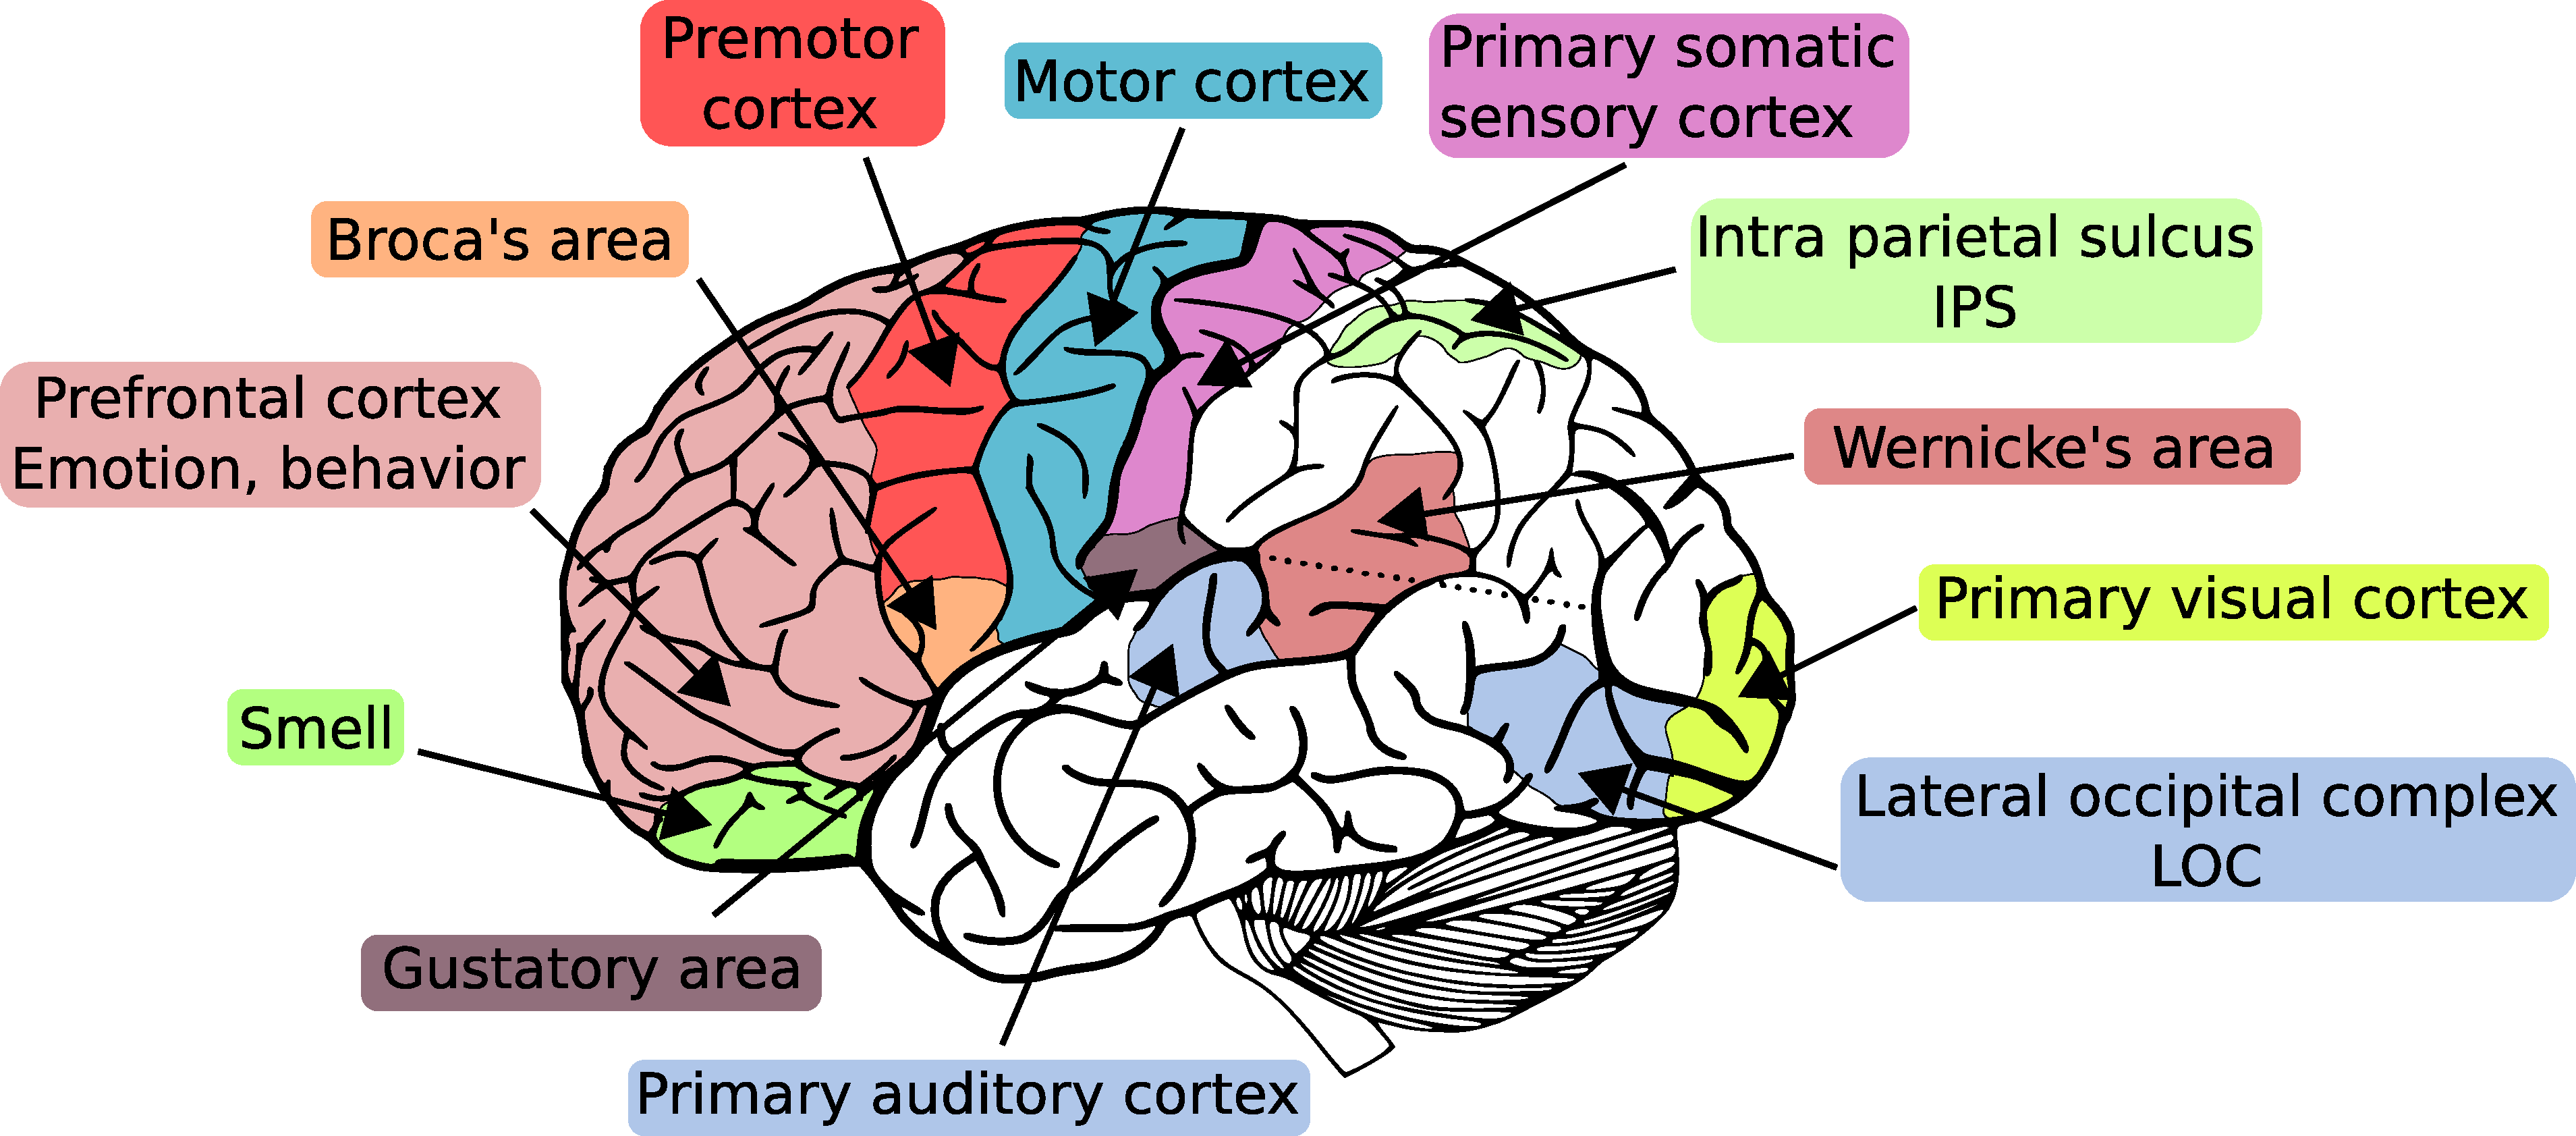
\includegraphics[width=1.\linewidth]{chapter_1/chapter_1_functions.pdf}
\end{center}
\caption{Lobes and some functional regions
of the human brain (left hemisphere).
Within each lobe are numerous cortical areas, each associated with a particular function such as
sensory areas (\emph{e.g. visual cortex, auditory cortex}) that receive and
process information from sensory organs, motors areas (\emph{e.g. primary motor
cortex, premotor cortex}) that control the movements of the subject,
and associative areas (\emph{e.g. Broca's area, Lateral Occipital Complex -- LOC
--
or Intra Parietal Sulcus -- IPS --}) that process the high-level information
related to cognition. The experiments detailed in this thesis are related to
object recognition (\emph{visual cortex} and \emph{LOC}) and number processing
(\emph{parietal cortex} and \emph{IPS}). Source: adapted from \citep{michel2010understanding}.}\label{fig:chapter_1_functions}. 
\end{figure}




\section{Functional neuroimaging modalities}

Until the advent in the 1920s of non-invasive neuroimaging modalities, most of the accumulated knowledge of the brain came from the study of lesions, post-mortem analysis and invasive experimentations. With the advent of modern, non-invasive imaging techniques, several aspects of the human brain are revealed in vivo with high degree of precision.

Several brain imaging techniques are available today. These can be divided into \emph{structural} or \emph{anatomical} and \emph{functional} imaging techniques. While structural imaging provides details on morphology and structure of tissues, functional imaging reveals physiological activities such as changes in metabolism, blood flow, regional chemical composition, and absorption. In this section we will discuss briefly the main functional neuroimaging modalities available today.

\begin{itemize}
\item{\bf {Electroencephalography - EEG}}
% \begin{marginfigure}[3cm]
% \center 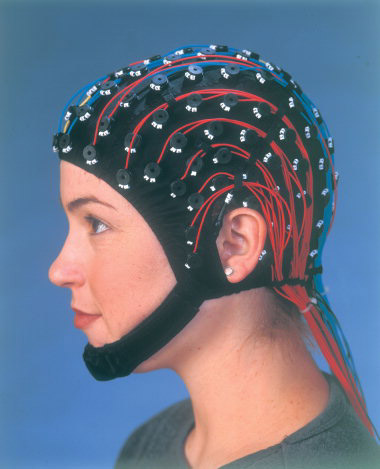
\includegraphics[width=.8\linewidth]{figures/eeg2.jpg}
% \caption{EEG Cap}
% \end{marginfigure}
is a widely used modality for functional brain
imaging. \emph{EEG} measures electrical activity along the scalp. EEG activity  reflects the synchronous activity of a population of neurons that have similar spatial orientation. If the cells do not have similar spatial orientation, their ions do not line up and thus do not create detectable waves. Pyramidal neurons of the cortex are thought to produce most of the EEG signals because they are well-aligned and fire together. Because voltage fields fall off with the square of distance, activity from deep sources is more difficult to detect than currents near the skull. Due to the ill-posed problem of
volumetric data reconstruction from surface measurements,
\emph{EEG} has a poor spatial resolution compared to other modalities
such as \emph{fMRI}.

\item{\bf {Stereotactic electroencephalography - sEEG}} is an invasive version of
\emph{EEG}, based on intra-cranial recording. It measures the electrical
currents
within some regions of the brain using deeply implanted electrodes, localized
with a stereotactic technique.
This approach has the good temporal resolution of \emph{EEG} and enjoys an
excellent spatial resolution. However, \emph{sEEG}
is very invasive and is only performed for medical purpose (\emph{e.g}
localization of epilepsy foci) and has a limited coverage (only the regions with electrodes).
A close approach is \emph{Electrocorticography -- ECog --} that uses
electrodes placed directly on the exposed surface of the brain. Even in this case its usage is restricted to medical purposes.


\begin{marginfigure}[5cm]
\center 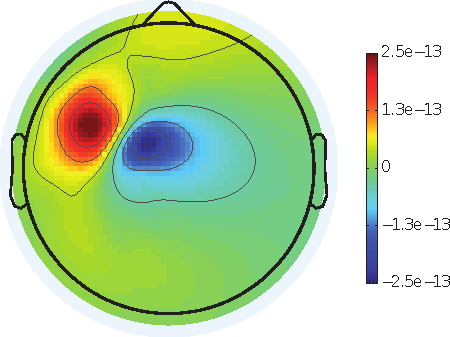
\includegraphics[width=1.\linewidth]{chapter_1/meg.pdf}
\caption{Magnetic field measured with MEG on a somato-sensory experiment. It is a 2D topography 20 ms after stimulation. Source: \citep{gramfort:09}}
\end{marginfigure}
\item{\bf{Magnetoencephalography - MEG}}
measures the magnetic field induced by neural electrical activity.
The synchronized currents in neurons create magnetic fields of a
few hundreds of femto Tesla ($fT$) that can be detected using specific devices. 
Although EEG and MEG signals originate from the same neurophysiological processes, there are important differences. Magnetic fields are less distorted than electric fields by the skull and scalp, which results in a better spatial resolution of the MEG. Whereas EEG is sensitive to both tangential and radial components of a current source in a spherical volume conductor, MEG detects only its tangential components. Because of this EEG can detect activity both in the sulci and at the top of the cortical gyri, whereas MEG is most sensitive to activity originating in sulci. EEG is, therefore, sensitive to activity in more brain areas, but activity that is visible in MEG can be localized with more accuracy. Note that EEG and MEG can be measured simultaneously.


\item{\bf{Positron emission tomography - PET}}
 is an imaging modality based on the
detection of a radioactive tracers introduced in the body of the subject. The
tracers (or \emph{radionuclide} decay) emit a positron which can in turn emit,
after recombination with an electron, a pair of photons that are detected
simultaneously. PET therefore provides a quantitative measurement of the physiological activity. It can also be used for functional imaging, by choosing a specific tracer.
In particular, the \emph{fluorodeoxyglucose} (or \emph{FDG}), is used for
imaging the metabolic activity of a tissue. This is based on the assumption that areas of high radioactivity are associated with brain activity.
\emph{PET} has two major limitations: the tracers required for
\emph{PET} are produced by cyclotrons (a type of particle accelerator),
which implies an heavy logistic. Furthermore, the use of radio-tracers is not harmless
for the
health of the subjects so \emph{PET} is now used for medical purpose only.

\begin{marginfigure}[0cm]
\center 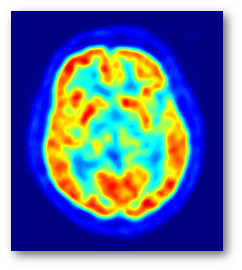
\includegraphics[width=.8\linewidth]{chapter_1/212px-PET-image.jpg}
\caption{PET scan of a human brain. 
PET measures indirectly the flow of blood to different parts of the brain, which is, in general, believed to be correlated with neural activity.
Souce: wikipedia.org}
\end{marginfigure}


\item{\bf{Single photon emission computed tomography - SPECT}} is an imaging modality based on the detection of a radioactive tracer. SPECT is similar
to \emph{PET} in its use of radioactive tracer material. However, the
measure in \emph{SPECT} is the direct consequence of the tracer (the tracer
emits gamma radiation), where \emph{PET} is based on an indirect consequence of
the tracer (positron then gamma radiation). The spatial resolution is slightly worse
than \emph{PET}.
%
\emph{SPECT} can be used for functional brain imaging, by using a specific
tracer which will be assimilated by the tissue in an amount proportional to
the cerebral blood flow.


\item{\bf{Near-infrared spectroscopy - nIRS}}
 is a recent modality for
medical imaging. \emph{nIRS} is based on the fact that the absorption of the
light in the
near-infrared domain contains information on the blood flow and blood
oxygenation level. It is non-ionizing (harmless), and the instruments are
not too expensive. However, the spectra obtained by \emph{nIRS} can be difficult
to interpret, and this technique, which requires a complex calibration, measures
signals only close to the outer layer of the cortex.

\newglossaryentry{fMRI}{name=fMRI,description=Functional Magnetic Resonance Imaging}

\item{\bf{Functional MRI} -- {\gls{fMRI}}} is
a widely used method for functional brain imaging, because it is
non-invasive, has a good spatial
resolution ($1mm^3$), and provides access,
albeit indirectly, to the neural activity.
Moreover, in standard acquisitions, \emph{fMRI} yields a
full-brain coverage, as it does not
restrict the study to superficial layers or predefined regions of the cortex.

\end{itemize}


Different modalities have different trade offs in terms of spatial and temporal resolution. For example, EEG and MEG enjoy temporal resolutions of the order of few miliseconds and are thus well suited for studies of temporal dynamics of information processing but have limited spatial resolution. On the other hand, fMRI enjoys a better spatial resolution but the temporal resolution is around 1 second. Furthermore, as we will see in the next section, temporal resolution in fMRI is further limited by the slow spread of hemodynamic response, which lasts around 20 seconds after the stimuli presentation.




\begin{figure}[h!tb]
\center 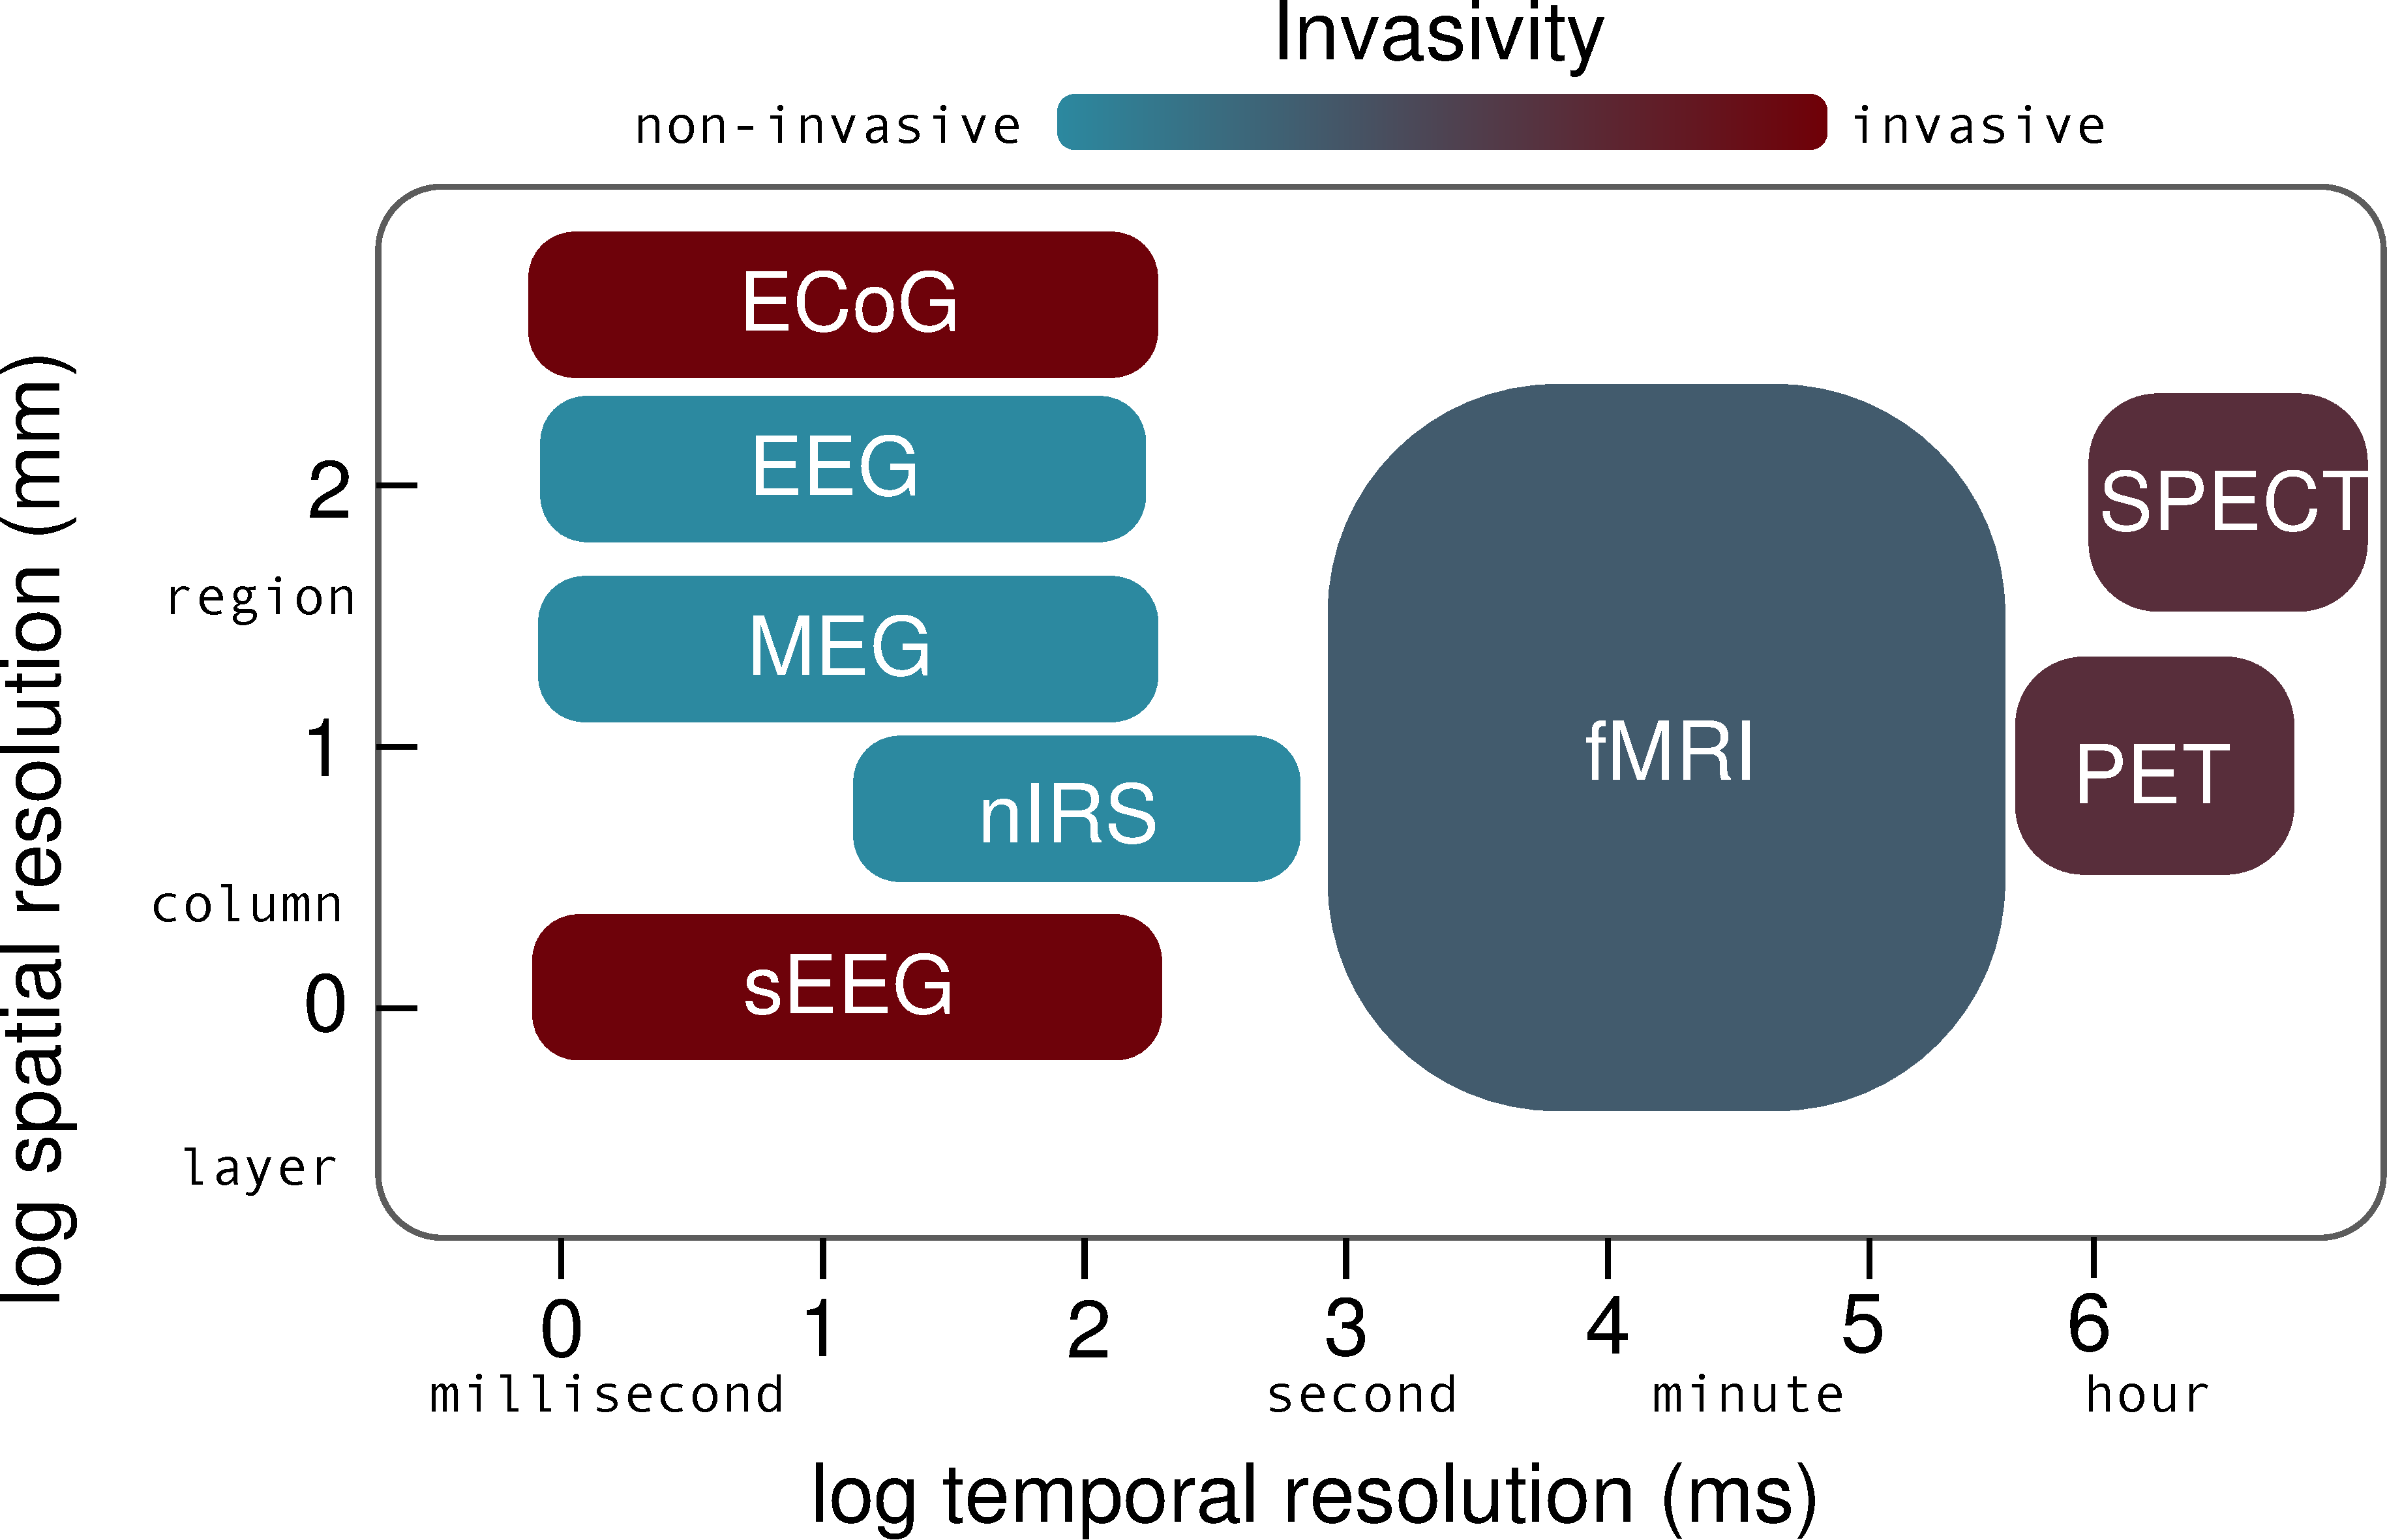
\includegraphics[width=0.8\linewidth]{chapter_1/chapter_1_methods.pdf}
\caption[Spatial and temporal resolutions of the different modalities commonly
used for functional imaging]{Spatial and temporal resolutions of different
modalities commonly
used for functional imaging. A typical fMRI acquisition (as of 2014) enjoys spatial resolution of the order of {$1-3mm^3$} and temporal resolution of the order of 1-3 seconds.}\label{fig:chapter1_methods}
\end{figure}

Certain imaging techniques are more adapted than other to answer certain neuroscientific questions. Due to its good spatial resolution and whole brain coverage, fMRI is particularly well adapted to \emph{localize} the effect of a certain experimental condition. This task is not reduced to the construction of brain maps, but also involves the understanding of the underlying brain connectivity~\citep{johansen2005functional,behrens2006consistent} and the effects regions exert on each other in a certain experimental context~\citep{pessiglione2007brain, behrens2007learning}. One of the main hopes in functional imagining is that it might be used as an objective diagnosis tool for several diseases. In particular, the aim is to find some \emph{biomarkers} for psychiatric diseases by comparing different population of patients: this is the case for autism, schizophrenia or Alzheimer's disease. 


\section{Functional MRI and BOLD signal}


\newglossaryentry{MRI}{name=MRI,description={{Magnetic Resonance Imaging}}}



The primary form of fMRI measures the oxygen change in blood flow. This is known as the Blood-oxygen-level dependent (BOLD) contrast. Other increasingly popular functional MRI method is arterial spin labeling (ASL)~\citep{detre1994tissue, alsop1998multisection, williams1992magnetic}, which uses arterial water as tracer to measure cerebral blood flow. Compared to fMRI, ASL has a lower signal to noise ratio~\citep{detre2002technical}. However, ASL provides reliable absolute quantification of cerebral blood flow with higher spatial and temporal resolution than other techniques~\citep{borogovac2012arterial}. This thesis specifically considers BOLD functional MRI and through the manuscript we use the name functional MRI (fMRI) to denote functional MRI based on the BOLD signal.

\newglossaryentry{bold}{name=BOLD,description={{fMRI contrast that measures oxygen change in blood flow}}}

%
The \emph{\gls{bold}} contrast can be explained by considering a protein present in
the blood
cells, called hemoglobin. Hemoglobin can bind with oxygen in order to bring it
into the different cells of the organism, this link being reversible and
unstable. Thus, it can be found in two different forms: \emph{oxyhemoglobin}
($Hb-O_{2}$ - giving a bright red color to the blood), its oxygenated form, and
\emph{deoxyhemoglobin} ($Hb$ - giving a blue-purple color to the blood), its
deoxygenated form.
%
%
%
%
When the \emph{oxyhemoglobin} loses its oxygen atoms and
becomes the \emph{deoxyhemoglobin}, it becomes more affected by an externally applied magnetic field (due to the iron
oxides). The presence of
\emph{deoxyhemoglobin} in the blood modifies the
magnetic resonance signal of the protons of the water molecules surrounding the blood
vessels. 

\begin{figure}
\centering
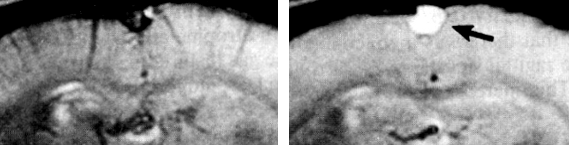
\includegraphics[width=1.\linewidth]{chapter_1/chapter_1_bold.png}
\caption[][-2.5cm]{
Illustration of the effect of the $CO_2$ on the \emph{BOLD} contrast.
Left - Coronal slice showing the \emph{BOLD} contrast of an anesthetized rat
which has breathed pure $O_2$. Right - Coronal slice of the same rat, showing the \emph{BOLD} contrast after respiration of a mixture of $90\%$ of $O_2$ and $10\%$ of $CO_2$ (this mixture
increases the oxygenation of the venous blood). The arrow shows 
the sagittal sinus, which is one of the major veins of the brain. This picture shows a strong increase of intensity in this vein, that illustrates that the
variation of blood oxygenation is visible in \emph{BOLD} contrast.
Adapted from \citep{ogawa1990b}.}\label{fig:chapter_1_ogawa}
\end{figure}


The difference of magnetic
susceptibility between the
blood vessel and the surrounding tissues creates 
inhomogeneities in the magnetic field \citep{thulborn1982,ogawa1990a} that are quantified by the magnetic resonance scanner. In the seminal paper \citep{ogawa1990b} studied the variations of
\emph{BOLD} contrast in the brain of an anesthetized rat during the inhalation of a gas
 that increases the \emph{cerebral blood flow} (\emph{CBF}), and thus blood
oxygenation (see Figure
\ref{fig:chapter_1_ogawa}).

\newglossaryentry{voxel}{name={voxel},description={unity of measure in a volumetric space}}
\newglossaryentry{TR}{name={TR},description={repetition time, sampling time in an fMRI scanner}}

The spatial resolution is given by the size of a \emph{\gls{voxel}}, a three-dimensional rectangular cuboid given by a single measure of the scanner. Voxel sizes range from 4mm to 1mm. Smaller voxels contain fewer neurons on average, incorporate less blood flow and hence have less signal to noise ratio than larger voxels. Smaller voxel size also makes up for longer acquisition time since this is proportional to the number of voxels per slice and the number of slices to scan. 

The time resolution of an fMRI scanner is given by the repetition time (\gls{TR}) of successive image acquisitions. A slice of the volume acquisition has an acquisition window that is about 20-30ms in duration. For example, in the study~\citep{borghesani:hal-00986606} we used voxel sizes of $1.5 \times 1.5 \times 1.5$mm, 82 slices and a repetition time (TR) of 2.3 seconds for a full-brain coverage. These number are for routine fMRI, however it is possible to change the tradeoff between spatial and temporal resolution. With the advent of compressed sensing techniques for faster acquisition times~\citep{MRM:MRM21391, Zong2014312, chauffertvariable} and the deployment of scanners with fields of 7-Tesla and beyond~\citep{hanke2014high} these numbers are likely to change in the near future.

% The dynamics, location, and magnitude of the signal are highly influenced by the vasculature as it is sampled in each voxel. If a voxel happen to capture large vessel effects, the magnitude of the signal may be larger, the timing a bit more delayed than average (up to 4 s delayed from capillary effects)~\citep{bandettini2009functional}









\section{Estimation of activation coefficients}\label{chapter1_activation_maps}


In this section we present a model that allows to extract time-independent \gls{activation coefficient}s relative to a given task given the BOLD time course and an experimental design. This model is known as the \emph{general linear model}~\citep{Friston1995}. We start by describing the \emph{hemodynamic response function} (Section~\ref{subsec:hrf}) and then describe an assumption behind the general linear model, the linear-time-invariant property (Section~\ref{subsec:lti}) between the BOLD signal and the neural response. The general linear model is then presented in Section~\ref{chapter_1_GLM}.


% fMRI acquisitions consist of successive brain scans, given in intervals ranging from 1 to 4 seconds. However, the methods that we consider in this thesis take as input time-independent \gls{activation coefficient}s relative to a given task. In this section we describe a method that allows to estimate time-independent \gls{activation coefficient} given the BOLD time course

% . 


The concepts presented in this section will form the basis of the contribution presented in Chapter~\ref{chap:hrf_estimation}, where we present an extension of the general linear model that performs the joint estimation of HRF and activation coefficients. 

Because it will not be referenced in later chapters we do not mention several \emph{preprocessing} steps that can be applied to the BOLD signal in order to remove artifacts that might have occurred during acquisition or to enhance the signal to noise ratio. These include slice-timing correction, motion correction, spatial normalization and spatial smoothing.


\subsection{Hemodynamic response function (HRF)}\label{subsec:hrf}
\newglossaryentry{HRF}{name=HRF,description=Hemodynamic Response Function}

One of the difficulties associated with fMRI studies is that BOLD signal does not increase instantaneously after the stimulus presentation nor does it return to baseline immediately after the stimulus ends. Instead, the BOLD signal peaks approximately 5 seconds after stimulation, and is followed by an undershoot that lasts as long as 30 seconds.

The \emph{Hemodynamic Response Function} (\gls{HRF}) represents an ideal, noiseless response to an infinitesimally brief stimulus. Most software packages represent the HRF as a sum of two gamma probability density functions, where the first gamma probability density function models the shape of the initial stimulus response and the second gamma probability density functions models the undershoot. Its analytical form is
\begin{equation}
h(t) = \frac{t^{\alpha_1 - 1} \beta_1^{\alpha_1} e^{-\beta_1 t}}{\Gamma(\alpha_1)} - 
c \frac{t^{\alpha_2 - 1} \beta_2^{\alpha_2} e^{-\beta_2 t}}{\Gamma(\alpha_2)}
\end{equation}
where $\Gamma$ is the gamma function and $\alpha_1, \alpha_2, \beta_1, \beta_2$ control the shape and scale, respectively, and $c$ determines the ratio of the response to undershoot.

\begin{figure}
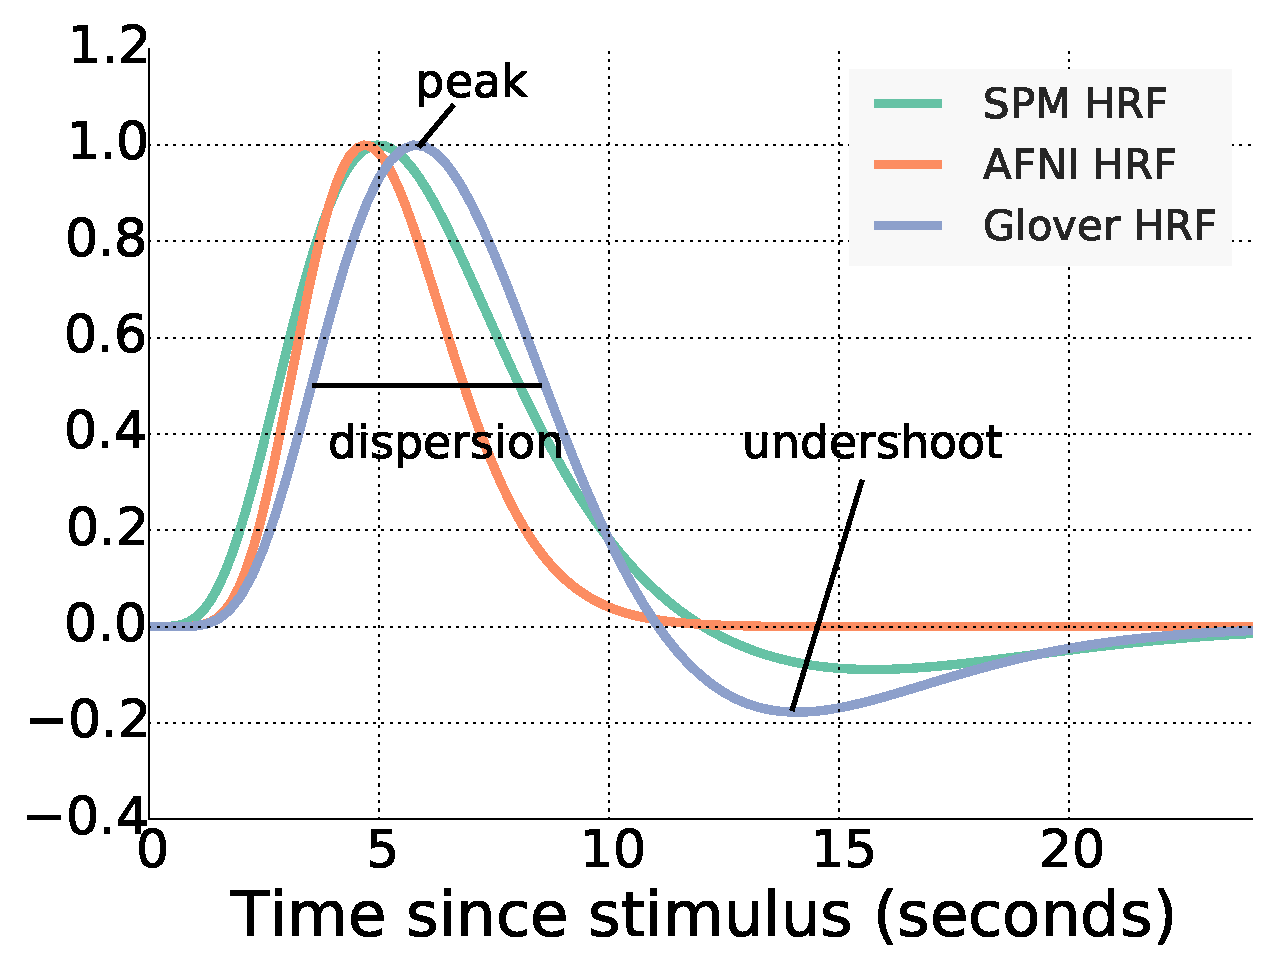
\includegraphics[width=1.\linewidth]{figures/chapter_1/canonical_hrf.pdf}
\hspace{-20pt}\caption{Hemodynamic Response Function (HRF) as implemented in different software packages. AFNI provides an HRF with no undershoot, i.e. modeled as a single gamma probability density function and where the peak is situated at 4.6 seconds. The software SPM provides an HRF that peaks at 5 seconds. \citet{Glover1999} proposes two models of the HRF, one based on a motor task and another based on an auditory task. Here we show the HRF corresponding to the auditory task since this is the one that is used in the software NiPy.}\label{fig:hrf_models}
\end{figure}

\newglossaryentry{reference HRF}{name=reference HRF,description=A particular HRF used in a software package.}



All the packages that we have considered model the HRF as the different of two gamma probability density functions but other models are equally possible. For instance, ~\citep{lindquist2009modeling} proposes the use of a model based on the superposition of three inverse logit functions.


\citet*{Glover1999} proposed two different sets of parameters based on the shape of the HRF on two different experiments. The parameters that are commonly used in statistical software such as \href{http://www.math.mcgill.ca/keith/fmristat/}{FMRISTAT}\footnote{\href{http://www.math.mcgill.ca/keith/fmristat/}{http://www.math.mcgill.ca/keith/fmristat/}} and \href{http://nipy.org}{NIPY}\footnote{\href{http://nipy.org}{http://nipy.org}} correspond to the HRF estimated in the auditory task. Its first gamma function peaks at 5.2 seconds, while the second gamma function (the undershoot) peaks at 12.2 seconds and has an amplitude of 35\% of the first gamma function. 

% This model has widely been shown to be successful at detecting fMRI activations and has been used extensively {\blue CITATION NEEDED}.


In the SPM\footnote{\href{http://www.fil.ion.ucl.ac.uk/spm/}{http://www.fil.ion.ucl.ac.uk/spm/}} software, the reference HRF has its peak at 6 seconds and the delay of undershoot has its minima at 16 seconds. AFNI\footnote{\href{http://afni.nimh.nih.gov/afni/}{http://afni.nimh.nih.gov/afni/} } on the other hands uses $c = 0$, that is, uses a model with a single gamma  distribution. A comparison of these different HRF models can be seen in Figure~\ref{fig:hrf_models}. Because of its widespread use, we will use the HRF present in SPM 8 unless otherwise specified.




\newglossaryentry{activation coefficient}{name={activation coefficient},description={amplitude for a single voxel associated with a stimuli in an fMRI study}}


\subsection{The linear-time-invariant assumption}\label{subsec:lti}

\newglossaryentry{LTI}{name=LTI,description=Linear Time Invariant assumption}

In this section we present the main assumption behind the general linear model, the \emph{linear time invariance} assumption.

A number of studies
have reported that in certain regimes the relationship between the neural response and the BOLD signal exhibits~\emph{linear time invariant} (\gls{LTI}) properties~\citep{Boynton1996,Cohen1997,Dale1997}. These property can be summarized as
\begin{itemize}
\item {\bf Multiplicative scaling}. If a neural response is scaled by a factor of $\alpha$, then the BOLD response is also scaled by a factor of $\alpha$.
\item {\bf Additivity}. If the response to two separate events is known, the signal for those events if they were to occur close in time is the sum of the independent signals.
\item {\bf Time invariant}. If the stimulus is shifted by $t$ seconds, the BOLD response will also be shifted by this same amount.
\end{itemize}

While the LTI assumption is commonplace in practice, there is evidence for non-linearity in the amplitude of the BOLD response. For example, it is known that there is a saturation effect for stimuli that occur less than 2 seconds apart~\citep{Wager2005206}. It has also been reported that very brief stimuli exhibit a larger BOLD response than would be expected based on longer stimuli~\citep{Yesilyurt2008853}. However, while these nonlinearities are important, there is a general consensus that for the range in which most cognitive fMRI studies occur, they will have relatively small impact.

\begin{figure}
\centering 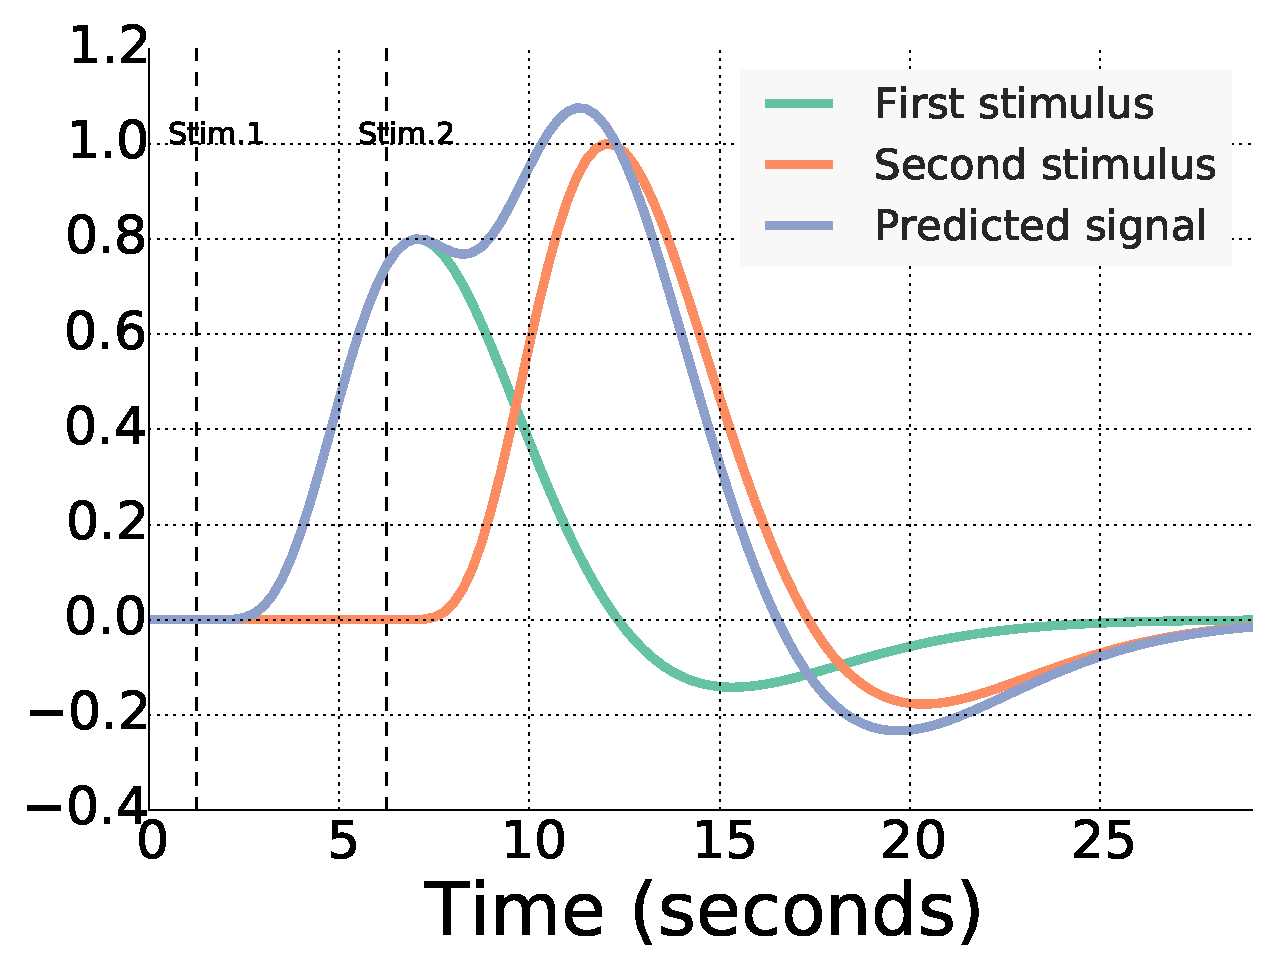
\includegraphics[width=.8\linewidth]{figures/chapter_1/linear_hrf.pdf}
\caption{The linear time invariant (LTI) assumption implies that if the response to two separate events is known, the signal for those events if they were to occur close in time is the sum of the independent signals. In green, the response to the first stimulus that is located at 1 second. In orange, the response to the second stimulus that appears at 6 seconds. In blue, the predicted BOLD response.}\label{fig:lti_hrf} 
\end{figure}



\newglossaryentry{conditions}{name={conditions},description={different stimuli in an fMRI study}}
\newglossaryentry{GLM}{name={GLM},description={General Linear Model}}



Let $x(t)$ represent the predicted BOLD arising from neuronal activity as a function of time $t$ and $h(\tau)$ be some reference HRF. The LTI assumption allows to easily construct the predicted BOLD response for a given stimulus function $u(t)$ which encodes the presence or absence of a stimulus (defined as one whenever the stimulus is present and zero otherwise). Then we can express the predicted BOLD (up to a constant factor) as the convolution of the stimulus function $u(t)$ with the HRF:
\begin{equation}
x(t) = \int_{0}^T\!u(t - \tau) h(\tau) \mathrm{d}\tau
\label{eq:chap1_predicted_bold}
\end{equation}

\subsection{The general linear model (GLM)}\label{chapter_1_GLM}


The General Linear Model (\gls{GLM}) makes use of the knowledge of the hemodynamic response function and linear-time-invariant assumption to model the observed BOLD signal. This model states that the BOLD signal can be expressed in terms of a linear combination of the predicted fMRI responses for different stimuli (also denoted \gls{conditions}) plus a noise term. Let $\{x_1(t), x_2(t), \ldots, x_k(t)\}$ be the predicted response for $k$ different stimulus functions computed from Equation~\eqref{eq:chap1_predicted_bold}. We define the design matrix $\B{X}$ as the columnwise stacking of different regressors, each one defined as the discretization of $x_i(t)$ to match the acquisition time of a given BOLD signal. The GLM in its basic form can be expressed as:
\begin{equation}
\begin{aligned}
\B{y} = \B{X}\bfbeta + \bvarepsilon \\
\bvarepsilon \sim \mathcal{N}(0, \sigma^2 \B{I})
\end{aligned}
\label{eq:chapter_1_glm}
\end{equation}
where $\B{y} \in \RR^n$ is the observed time course at a single voxel, $\bfbeta \in \RR^k$ is the activation coefficients that represent the amplitude of the response for a given condition and $\bfvarepsilon$ is a noise term that we assume Gaussian for now (we will see in Section~\ref{subsec:prewhite} how to take into account temporal autocorrelation). 
\begin{figure*}[t]
\center 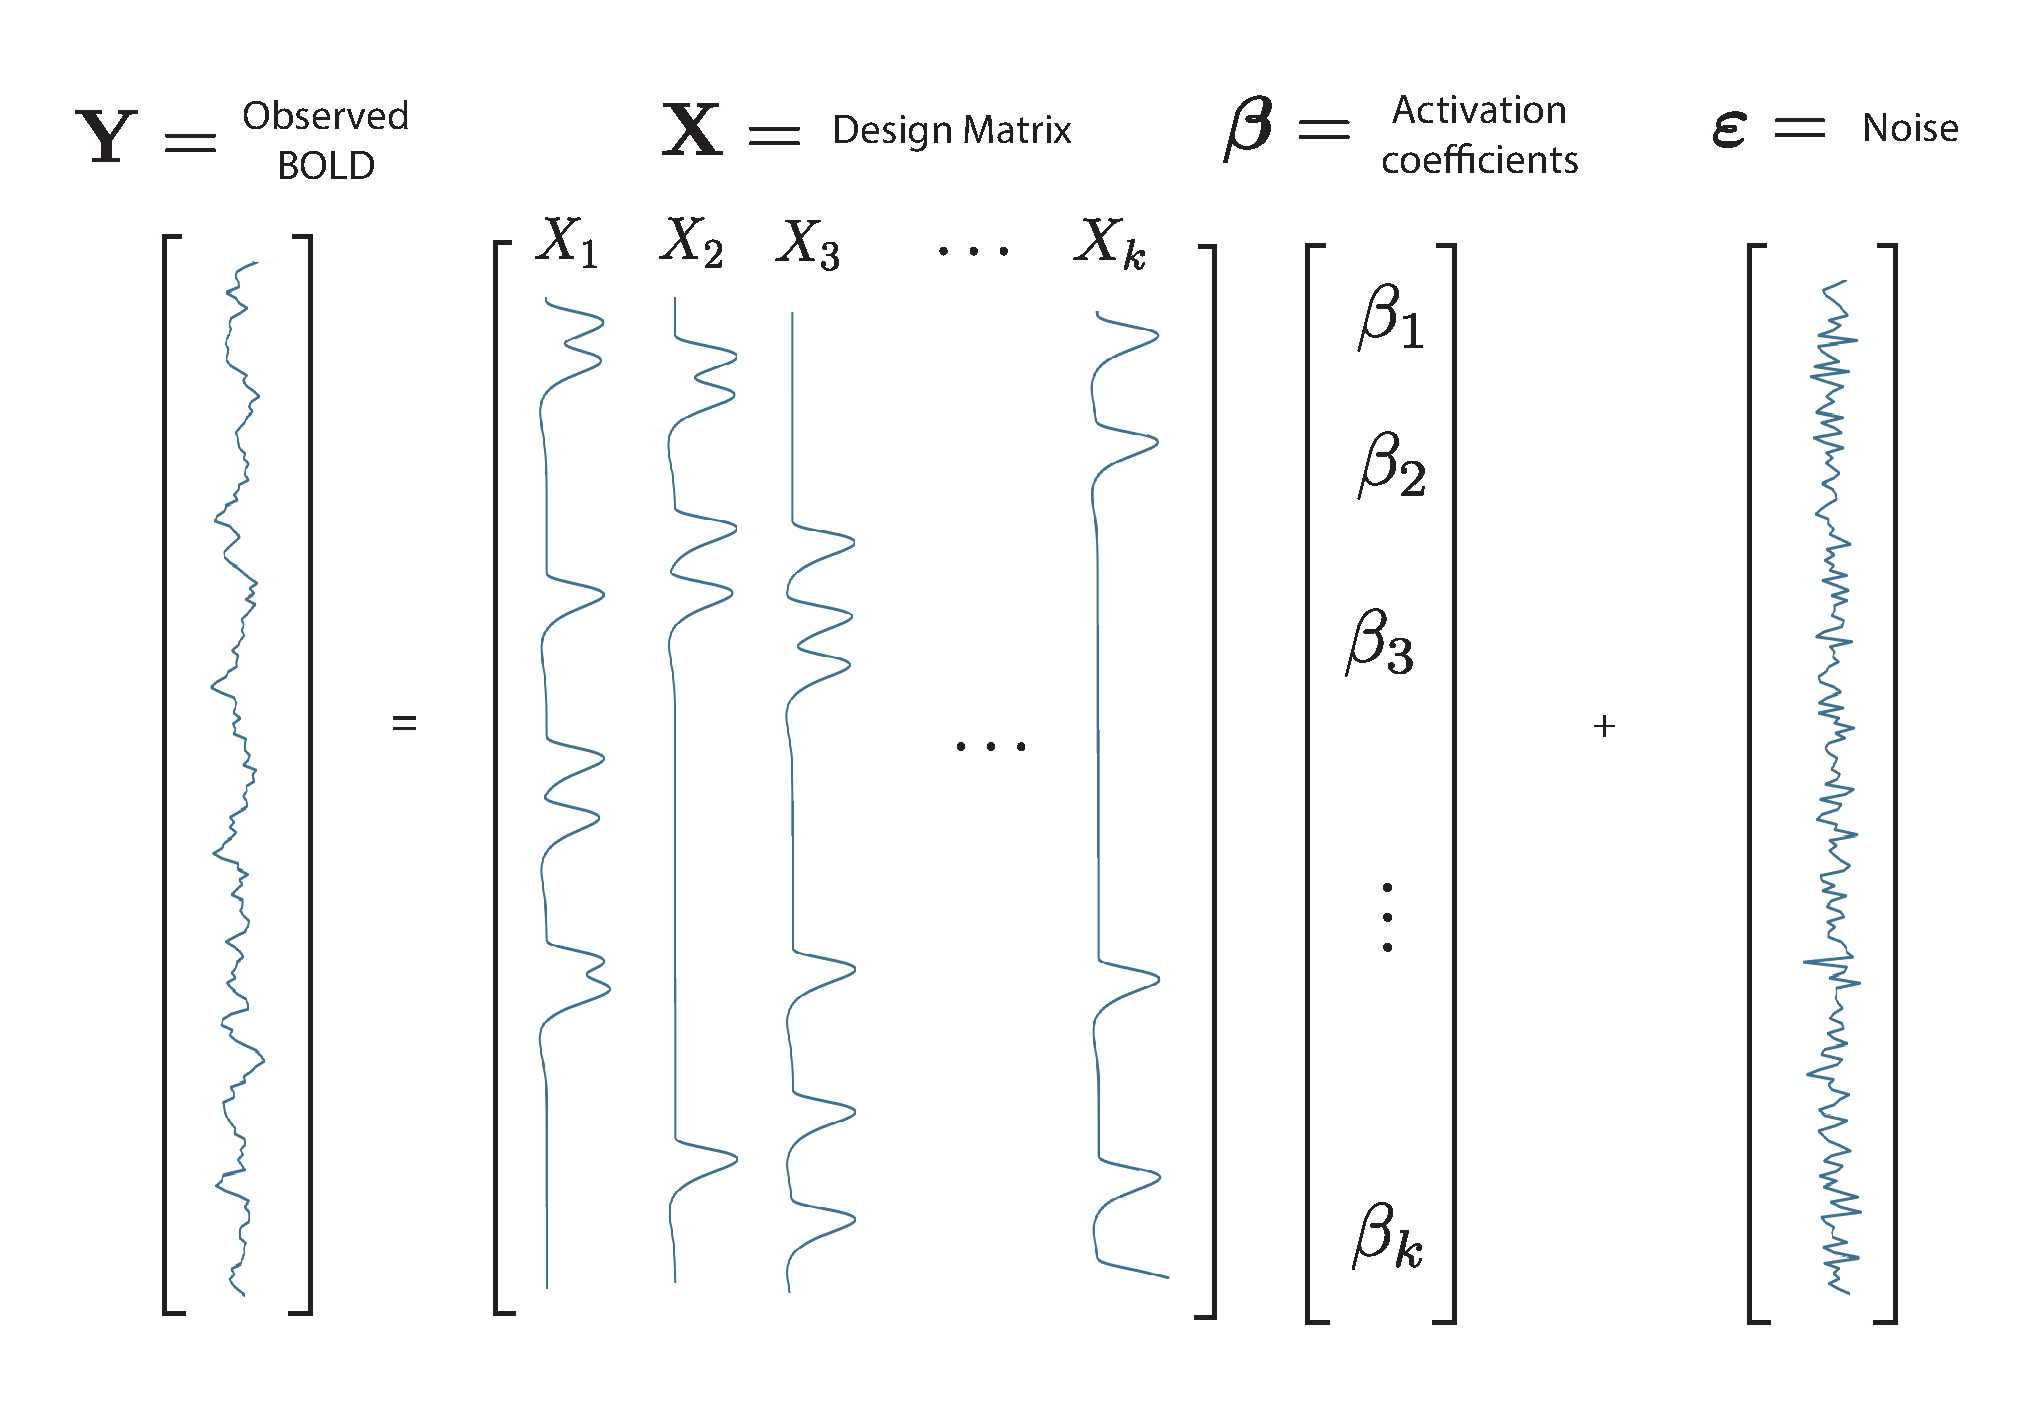
\includegraphics[width=.8\linewidth]{figures/chapter_1/glm_plain.pdf}
\caption{The GLM expresses the observed BOLD signal as a linear combination of regressors plus an error term. Each regressor of the design matrix is the convolution of a reference HRF and the stimulus function, a function that is 1 when the stimulus is present and zero otherwise. Each element of the (unknown) activation coefficients represent the relative amplitude of a given condition.}\label{fig:glm1}
\end{figure*}


Assuming Gaussian i.i.d noise, the maximum likelihood estimation of the activation coefficients is then given by $\hat{\bfbeta} = \argmin_{\bfbeta}\|\B{y} - \B{X}\bfbeta \|^2 = \B{X}^{\dagger} \B{y}$. To estimate the activation coefficients in a full brain volume this procedure is repeated independently for each voxel. Since the design matrix is the same across voxels, a matrix decomposition of $\B{X}$ such as SVD or QR can be computed once and then used to compute the least squares solution at every voxel.


In this setting we have considered the HRF to be known and fixed across the different conditions. We can easily generalize this setting to accommodate the case in which the HRF is generated by a given basis set. We will call this method \emph{basis-constrained GLM}.


\subsection{High-pass filtering and prewhitening}\label{subsec:prewhite}

The BOLD signal contains low frequency trends that are usually removed before or during the estimation of activation coefficients. One popular approach of high-pass filtering is to add a discrete cosine transform (DCT) basis set to the design matrix. When using this basis set, the highest frequency that is desired to be removed from the data has to be chosen to avoid removing the frequency of the experimental task that is also being modeled. Another approach that is becoming increasingly popular, is to fit a local regression model to the time series and remove the estimated trend from the data. The software FSL uses LOWESS (locally weighted scatterplot smoothing)~\citep{cleveland1979robust} while recent studies have successfully used a Savizky-Golay filter
\sidenote{Savitzky-Golay filter are available in Matlab under the name \texttt{\small sgolayfilt} and in Python's Scipy module under the name \texttt{\small scipy.signal.savgol\_filter}}
\citep{barry2014enhanced,ccukur2013attention}. In the studies presented in Chapter 3 we will use this last filter.  In \citep{ccukur2013attention}, the authors used a Savizky-Golay filter to estimate the low-frequency drifts with window length of 240 seconds and polynomial of degree 3. We have found that parameters close to these work well in practice. 
\newglossaryentry{AR(1)}{name={AR(1)},description={autorregressive with variance 1}}


The GLM specified in~\eqref{eq:chapter_1_glm} assumes the noise $\bvarepsilon$ follows a Gaussian random variable with covariance $\sigma^2 \B{I}$. However, it is known that the BOLD signal is temporally autocorrelated. Several authors~\citep{bullmore1996statistical,kruggel2000nonlinear} consider the BOLD noise as an autoregressive model \emph{AR(1)}. This assumes each time point is correlated with the previous time point. The distribution of the error in this case is given by $\varepsilon \sim \mathcal{N}(0, \sigma^2 \B{V})$, where $\B{V}$ is the symmetric correlation matrix and $\sigma^2$ is the variance. The correlation matrix and variance are commonly estimated from the residuals after fitting the GLM. 

The most common solution to take this special structure into account is to \emph{prewhiten} the data, that is, to remove the temporal correlation. Since the correlation matrix $\B{V}$ is symmetric and positive definite, the Cholesky decomposition can be used to find a matrix $\B{K}$ such that $\B{V}^{-1} = \B{K}^T \B{K}$. To prewhiten the data, $\B{K}$ is premultiplied on both sides of the GLM (Eq.~\eqref{eq:chapter_1_glm}) to give $\B{K}\B{y} = \B{K}\B{X} \bfbeta + \B{K}\bfvarepsilon$. This makes the errors be independent, i.e., $\B{K}\bfvarepsilon \sim \mathcal{N}(0, \sigma^2 \B{I})$.


\section{Conclusion}
In this first chapter we have presented the principal structures of the human brain. We have then presented the principal functional imaging modalities in use today, with special emphasis on functional MRI. We have seen that functional MRI is an attractive modality for functional imaging with good spatial resolution for a whole brain coverage modality. The signal measured in fMRI studies is the BOLD signal, given in the form of a succession of scans in intervals of 1-4 seconds. The extraction of time-independent activation maps from the BOLD signal relies on the linear-time-invariant property between neural response and the BOLD signal. These can be estimated by solving a least-squares problem, a setting commonly referred to in neuroimaging as the \emph{general linear model} (GLM). The GLM is usually formulated using a known form of the Hemodynamic Response Function.

\newpage

\begin{fullwidth}
\bibliographystyle{plainnat}
\bibliography{chapter_1/biblio1}
\end{fullwidth}





